In this chapter, the \textit{SLDC} framework is applied the problem presented in Chapter \ref{chap:context} : the nodule malignancy assessment. This problem is effectively an instance of the objects detection and classification problem. Indeed, the goal is to diagnose malignancy by the presence or absence of cells or groups of cells having particular characteristics in digitized microscope whole-slide. This problem is a good use case for the \textit{SLDC} framework: the images are large (i.e. typically 15 giga-pixels), two distinct categories of objects must be found (namely cells and groups of cells) and some of these objects can be included into others which can be handled using dispatching and chaining.  

The implementation issues and challenges related to this particular problem are presented in Section \ref{sec:thyroid_impl_issue}. Then, as this problem was already addressed in \cite{adeblire2013}, the workflow developed in this work is briefly presented and assessed in Section \ref{sec:thyroid_adeblire_algo}. Especially, some flawed steps are highlighted and some improvements are proposed. 
Then, the implementation of the improved workfow is detailed in section \ref{sec:thyroid_implementation}. Finally, the performances of this implementation are assessed in Section \ref{sec:thyroid_perf}.

\section{Implementation issues}
\label{sec:thyroid_impl_issue}
To successfully solve the thyroid problem involves several technical challenges which are presented hereafter.

\subsection{Large images and networking}
The images on which must be applied the workflow are large. 

\subsection{Dataset} 
The detection part consists in finding those cells and grouping in the slides. 




Presentation of implementation issues related to the thyroid case (image size, over HTTP, image quality, human annotation vs computer annotation, presence of inclusions in patterns, dispatching ...)

\section{First workflow}
\label{sec:thyroid_adeblire_algo}

The workflow developed by Antoine Deblire in \cite{adeblire2013} is summarized in \ref{fig:workflow_adeblire}. The idea behind this workflow is fairly simple. A first segmentation is applied to extract standalone cells and architectural patterns (step 4.3). The detected objects are then differentiated using their area and circularity (step 4.4) and dispatched to a classifier (steps 4.6). Especially, the classifier for architectural patterns is supposed to classify them as proliferative or non-proliferative and the one for cells is supposed to detect whether they contain an inclusion or not. Then, architectural patterns are segmented again (step 4.5) to extract the cells they contain. Those cells are also passed to the cell classifier. 

\begin{figure}
	\center
	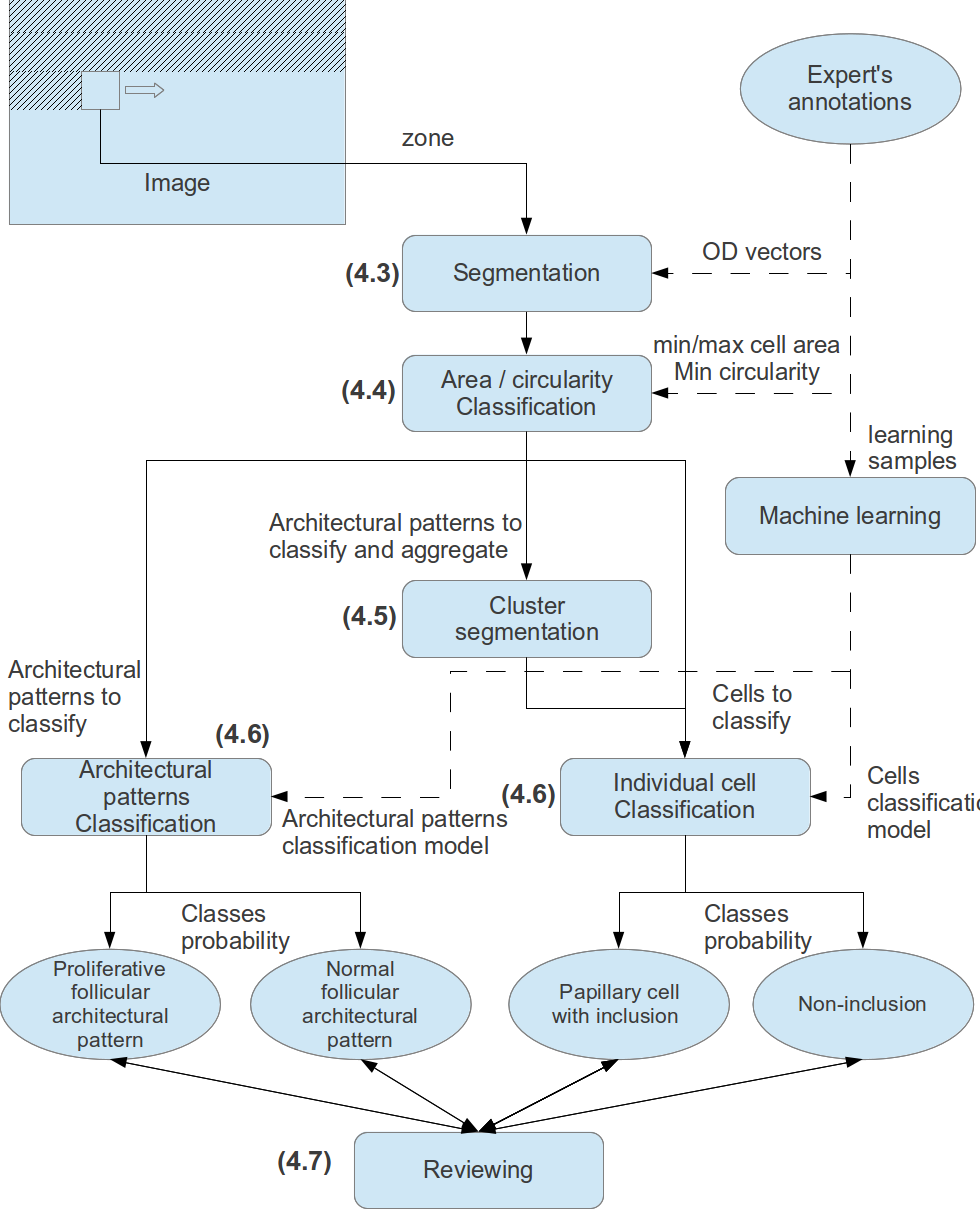
\includegraphics[scale=0.95]{image/adeblire_workflow.png}
	\caption{Antoine Deblire's workflow (source: \cite{adeblire2013})}
	\label{fig:workflow_adeblire}
\end{figure}

\subsection{Segmentation procedures}
The first segmentation procedure was designed for processing the whole slide and relies on a process called color deconvolution \cite{ruifrok2001quantification}. This process consists in retrieving the tissues stains concentration from the RGB image. In the context of this project, it appears that cells and patterns have a high concentration of a given stain. Therefore, a first segmentation mask is generated by thresholding this stain concentration image. Some morphological operations are then applied in order to remove noise and fill unwanted holes. Some example segmentations are provided in Figure \ref{fig:first_seg_examples}. It seems that the procedure is able to detect most of the objects of interest although it sometimes fails at covering the whole object area. For instance in the third example image, the present inside the pattern excludes from the binary mask the cell with inclusion. On the fourth example, one can see three standalone objects above the central pattern. Those objects' masks are smaller than their corresponding cells.

\begin{figure}
	\center
	\subfigure{
		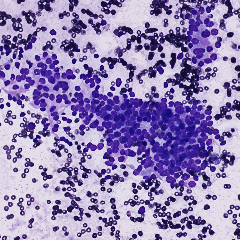
\includegraphics[scale=0.5]{image/slide_segmentation_0_in.png}
		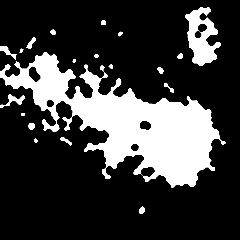
\includegraphics[scale=0.5]{image/slide_segmentation_0_out.png}
		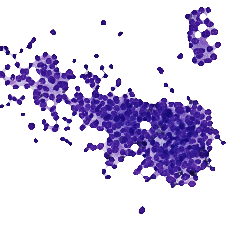
\includegraphics[scale=0.5]{image/slide_segmentation_0_masked.png}
	} \\
	\subfigure{
		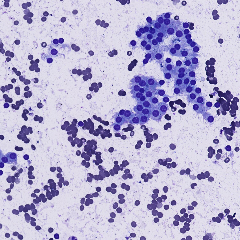
\includegraphics[scale=0.5]{image/slide_segmentation_1_in.png}
		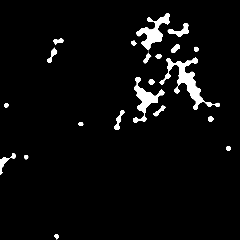
\includegraphics[scale=0.5]{image/slide_segmentation_1_out.png}
		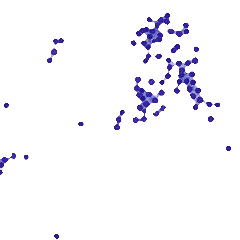
\includegraphics[scale=0.5]{image/slide_segmentation_1_masked.png}
	} \\
	\subfigure{
		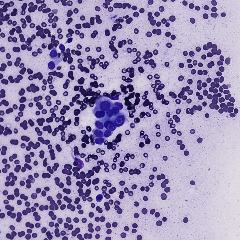
\includegraphics[scale=0.5]{image/slide_segmentation_2_in.png}
		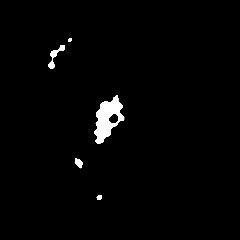
\includegraphics[scale=0.5]{image/slide_segmentation_2_out.png}
		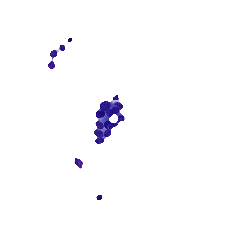
\includegraphics[scale=0.5]{image/slide_segmentation_2_masked.png}
	} \\
	\subfigure{
		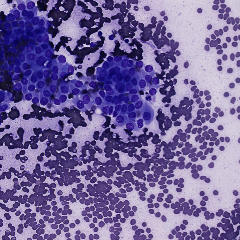
\includegraphics[scale=0.5]{image/slide_segmentation_3_in.png}
		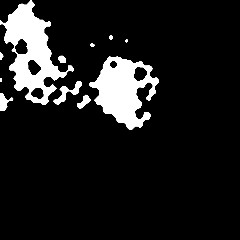
\includegraphics[scale=0.5]{image/slide_segmentation_3_out.png}
		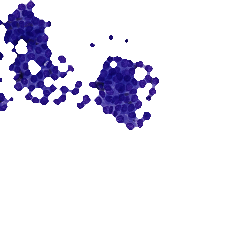
\includegraphics[scale=0.5]{image/slide_segmentation_3_masked.png}
	}
	\caption{First segmentation - examples}
	\label{fig:first_seg_examples}
\end{figure}

The second segmentation procedure is applied to the architectural patterns and is designed to isolate individual cells inside those patterns. The implementation is a little more complicated than the first. Similarly, it starts with a color deconvolution to highlight the cells. However, the stain concentration image is not transformed into a binary mask using a fixed threshold but using Otsu's method. Using the \texttt{findContour} procedure of the OpenCV library, independent cells are located and cleaned one after the other. Finally, a watershed algorithm is applied to separate cells that intersects. Some example segmentations are provided in Figure \ref{fig:first_seg_examples}. The segmentation seems to work relatively well on "clean" patterns, that is where cells doesn't overlap much and are clearly distinguishable from the pattern background (see the first two examples in Figure \ref{fig:first_seg_examples}). One "dirty" patterns however, the segmentation performs poorly as it returns large patches.  

\begin{figure}
	\center
	\subfigure{
		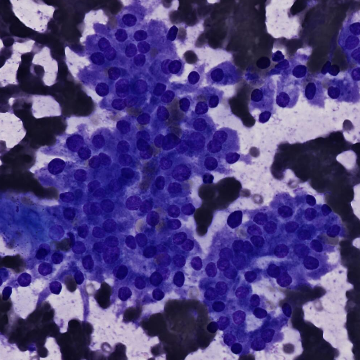
\includegraphics[scale=0.33]{image/aggr_segment_12_in.png}
		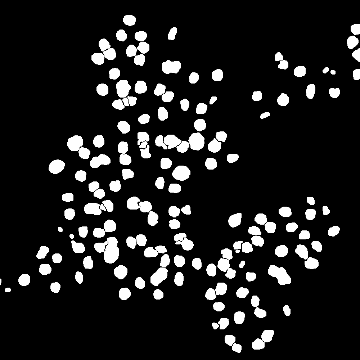
\includegraphics[scale=0.33]{image/aggr_segment_12_out.png}
		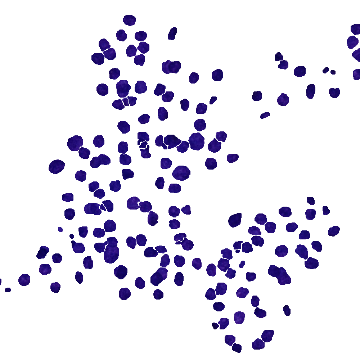
\includegraphics[scale=0.33]{image/aggr_segment_12_masked.png}
	} \\
	\subfigure{
		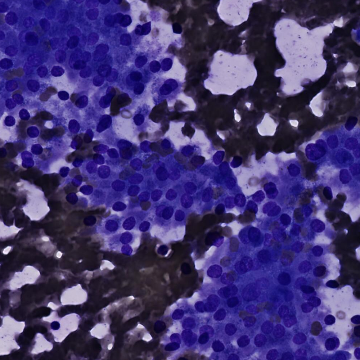
\includegraphics[scale=0.33]{image/aggr_segment_2_in.png}
		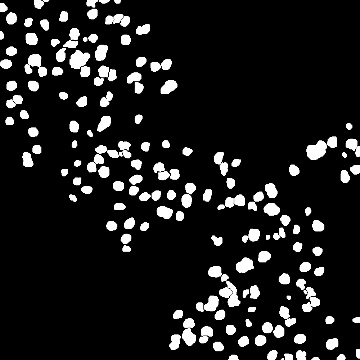
\includegraphics[scale=0.33]{image/aggr_segment_2_out.png}
		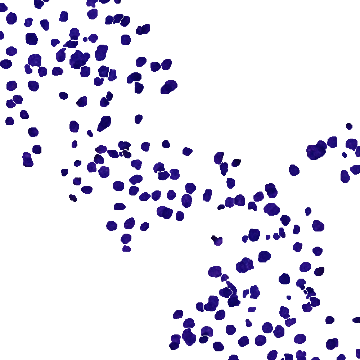
\includegraphics[scale=0.33]{image/aggr_segment_2_masked.png}
	} \\
	\subfigure{
		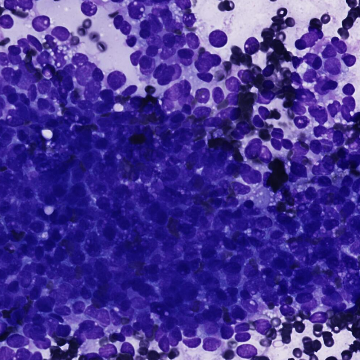
\includegraphics[scale=0.33]{image/aggr_segment_5_in.png}
		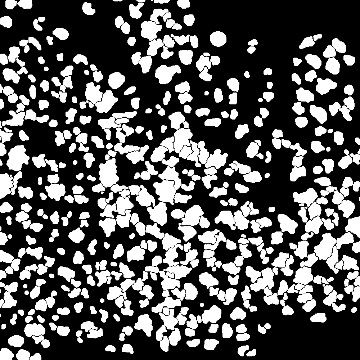
\includegraphics[scale=0.33]{image/aggr_segment_5_out.png}
		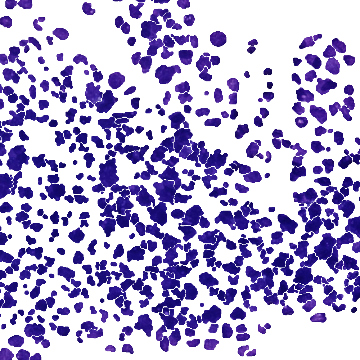
\includegraphics[scale=0.33]{image/aggr_segment_5_masked.png}
	} \\
	\subfigure{
		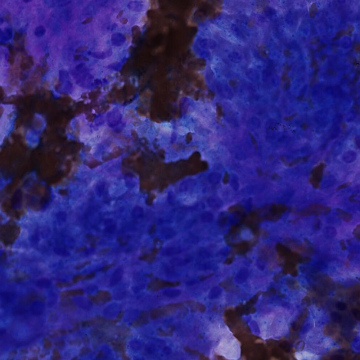
\includegraphics[scale=0.33]{image/aggr_segment_7_in.png}
		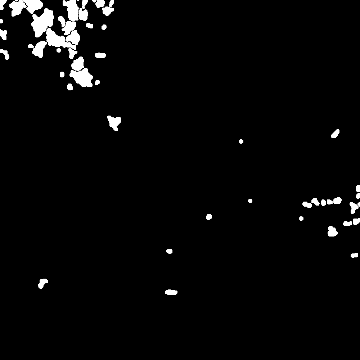
\includegraphics[scale=0.33]{image/aggr_segment_7_out.png}
		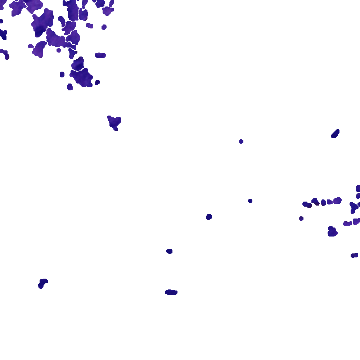
\includegraphics[scale=0.33]{image/aggr_segment_7_masked.png}
	}
	\caption{Second segmentation - examples}
	\label{fig:second_seg_examples}
\end{figure}

While the presented segmentation procedures exhibit some flaws, they were considered acceptable to test the  framework.

\subsection{Dispatching procedure}

The step (4.4) consisted in dispatching detected objects into four categories: artefacts, cells, clusters and patterns. The category \textit{artefact} corresponds to irrelevant objects and the category \textit{cluster} is a group of cells that contains too few of them to be pattern. Even if the author did distinguish patterns and clusters at the dispatching step, objects of both categories were treated equally in the subsequent steps of the algorithm. That is, they were first evaluated by the pattern classifier (for assessing whether they were proliferative or not) and then they were re-segmented. The dispatching was based on four parameters, the cell minimum and maximum areas (respectively, $A_{min}$ and $A_{max}$), the cell minimum circularity $C_{min}$ and the minimum number of cells per pattern $N_{min}$. The values of those parameters are given in Table \ref{tab:adeb_disp_rules}. 

Given $A$ the area of the object of interest, the dispatching rules can be summarized as follows:

\begin{itemize}
	\item \textbf{Artifact}: every object having an area less than $A_{min}$ or and area less than $A_{max}$ and a circularity less then $C_{min}$
	\item \textbf{Cell}: every object having an area such that $A_{min} < A < A_{max}$ and a circularity greater than $C_{min}$
	\item \textbf{Clusters}: every object of which the area is greater than $A_{max}$ and such that it contains at most $N_{min}$ cells:
	\[
		A_{max} < A < N_{min} \times A_{max}
	\]
	\item \textbf{Patterns}: all objects which don't match one of the rule above are considered patterns
\end{itemize}

\begin{table}
	\center
	\begin{tabular}{|c|c|}
		\hline
		$A_{min}$ & 31 $\mu m^2$\\
		\hline
		$A_{max}$ & 102 $\mu m^2$\\
		\hline
		$C_{min}$ & 0.7 \\
		\hline
		$N_{min}$ & 4\\
		\hline
	\end{tabular}
	\caption{Dispatching parameters presented in \cite{adeblire2013}}
	\label{tab:adeb_disp_rules}
\end{table}

As stated in \ref{adeblire2013}, the dispatching parameters were chosen based on the areas and circularities of the experts' annotations. While this source might provide a qualitative insight about the parameters values, they should not be used to determine the actual values. Indeed, experts usually annotate objects roughly which means that the annotation area will often be larger than the object's real area. Moreover, Cytomine provides several drawing tools, one of which for drawing a circle around a point. The usage of this tool results in a circularity close to 1 even if the underlying object is far from being circular.

Nonetheless, in order the assess whether the dispatching rules are effective for distinguishing cells from patterns, the expert annotations present on Cytomine were used. Indeed, in this case, only a qualitative analysis is performed. The histograms given in Figures \ref{fig:hist_area_cell_vs_pattern} and \ref{fig:hist_circ_cell_vs_pattern} respectively show the area and circularity distributions of the experts' annotations. First, it appears that, whatever the metric, there is a substantial overlapping between the cells' and patterns' distributions. This has a major consequence for the dispatching. Indeed, it breaks the rules presented above as they rely on a simple thresholding. Another observation is that the parameters given in Table \ref{tab:adeb_disp_rules} are not relevant as most of the cells would be dispatched as patterns with such values. This observation is confirmed with the scatter plot shown in Figure \ref{fig:scatter_area_circ_cell_vs_pattern}. In this chart, only few cells are effectively dispatched as such (the ones that fall into the blue box), the others being dispatched as patterns.


\begin{figure}
	\center
	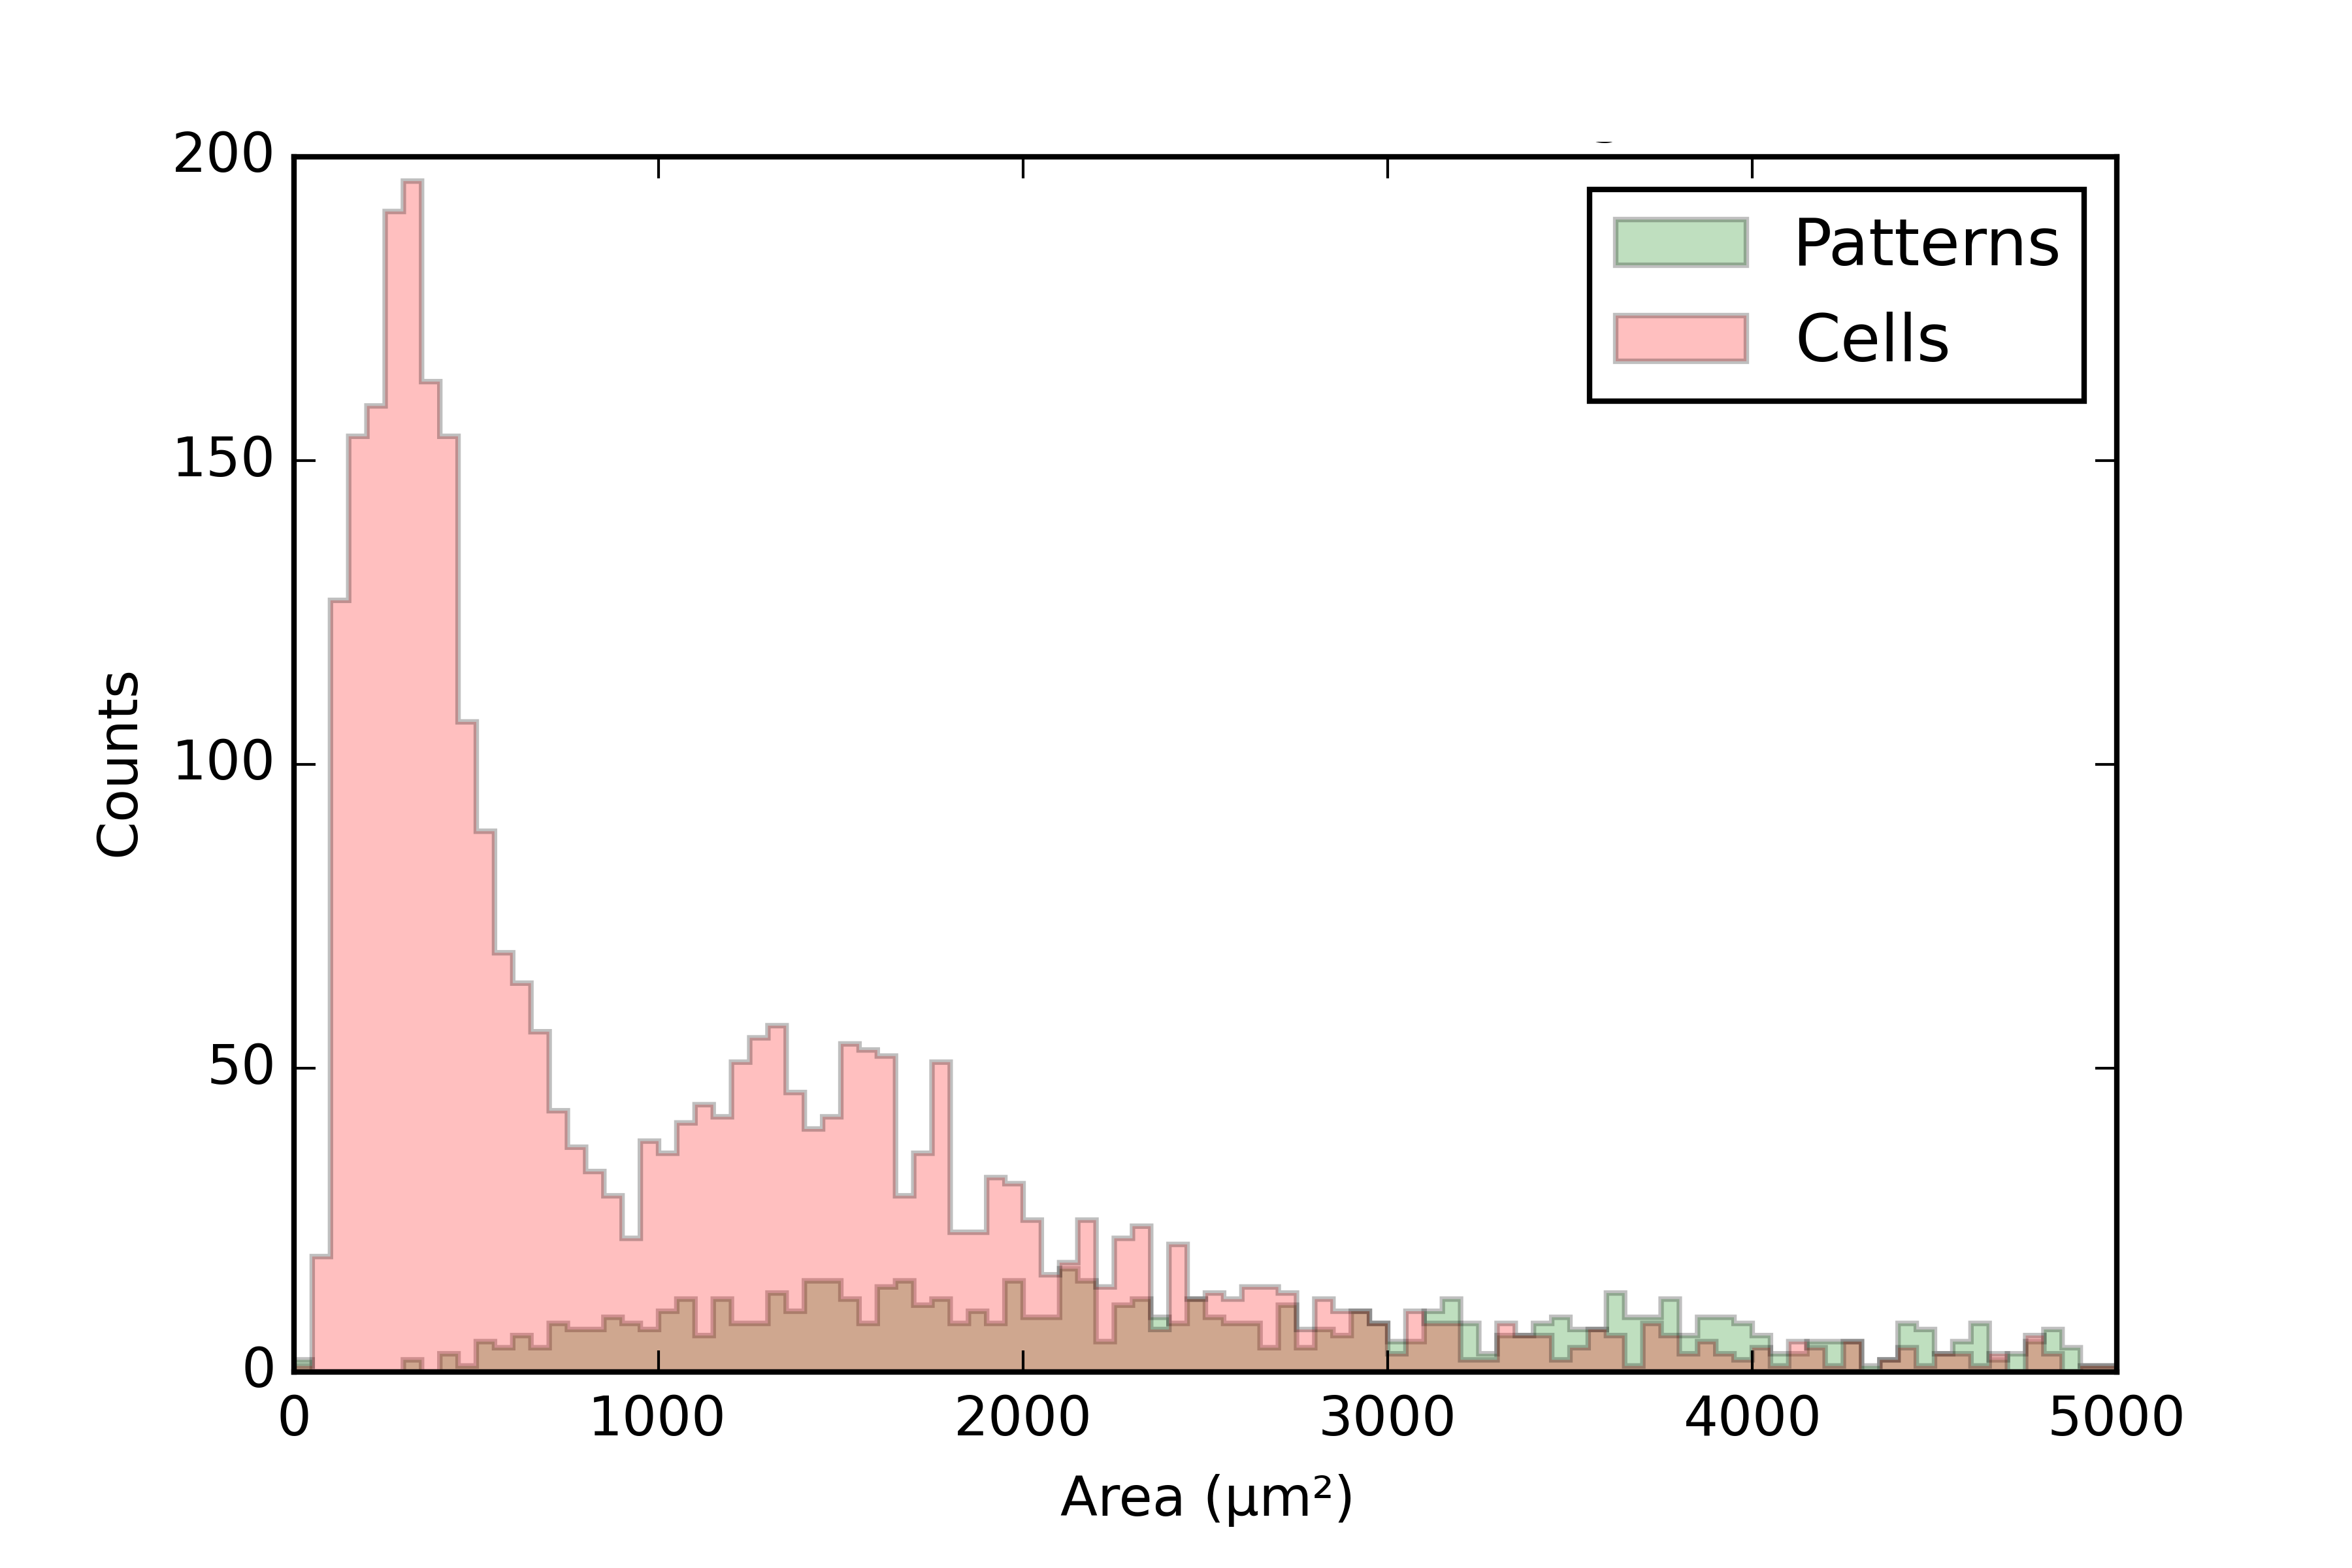
\includegraphics[scale=0.75]{image/cells_patterns_real_area_0_5000.png}
	\caption{Area distributions of the experts' annotations.}
	\label{fig:hist_area_cell_vs_pattern}
\end{figure}

\begin{figure}
	\center
	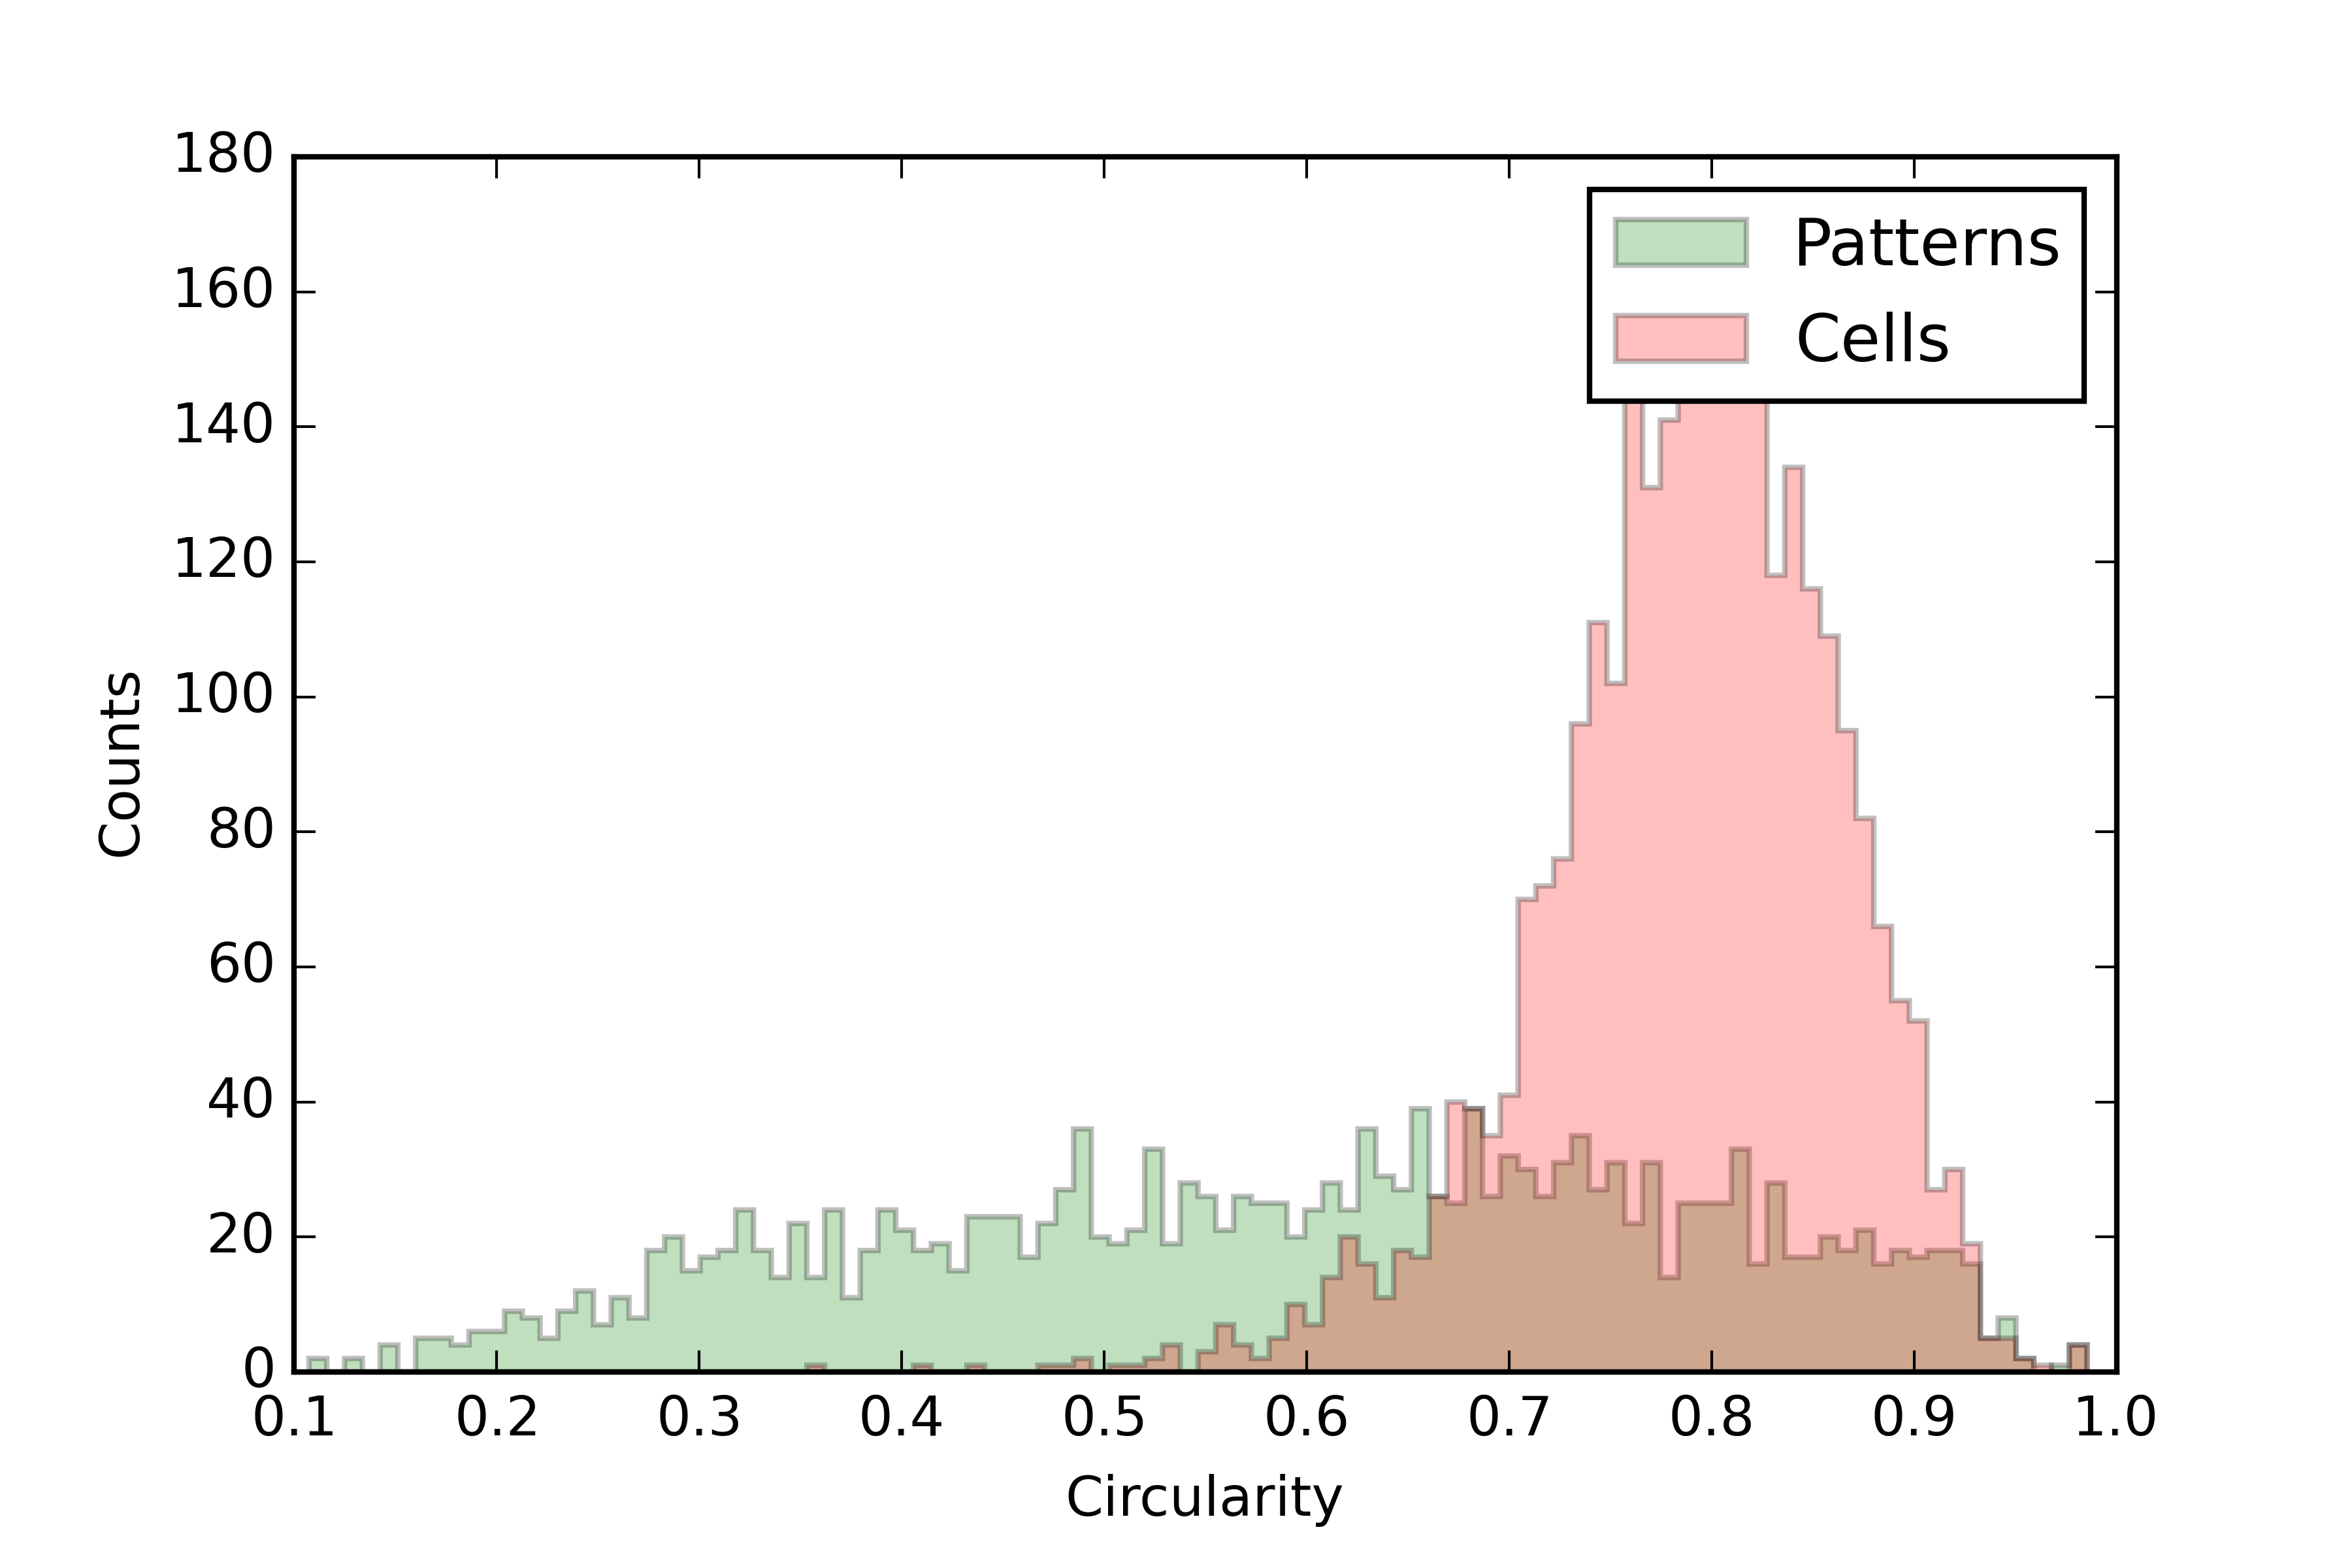
\includegraphics[scale=0.75]{image/cells_patterns_circ.png}
	\caption{Circularity distribution of the experts' annotations.}
	\label{fig:hist_circ_cell_vs_pattern}
\end{figure}

\begin{figure}
	\center
	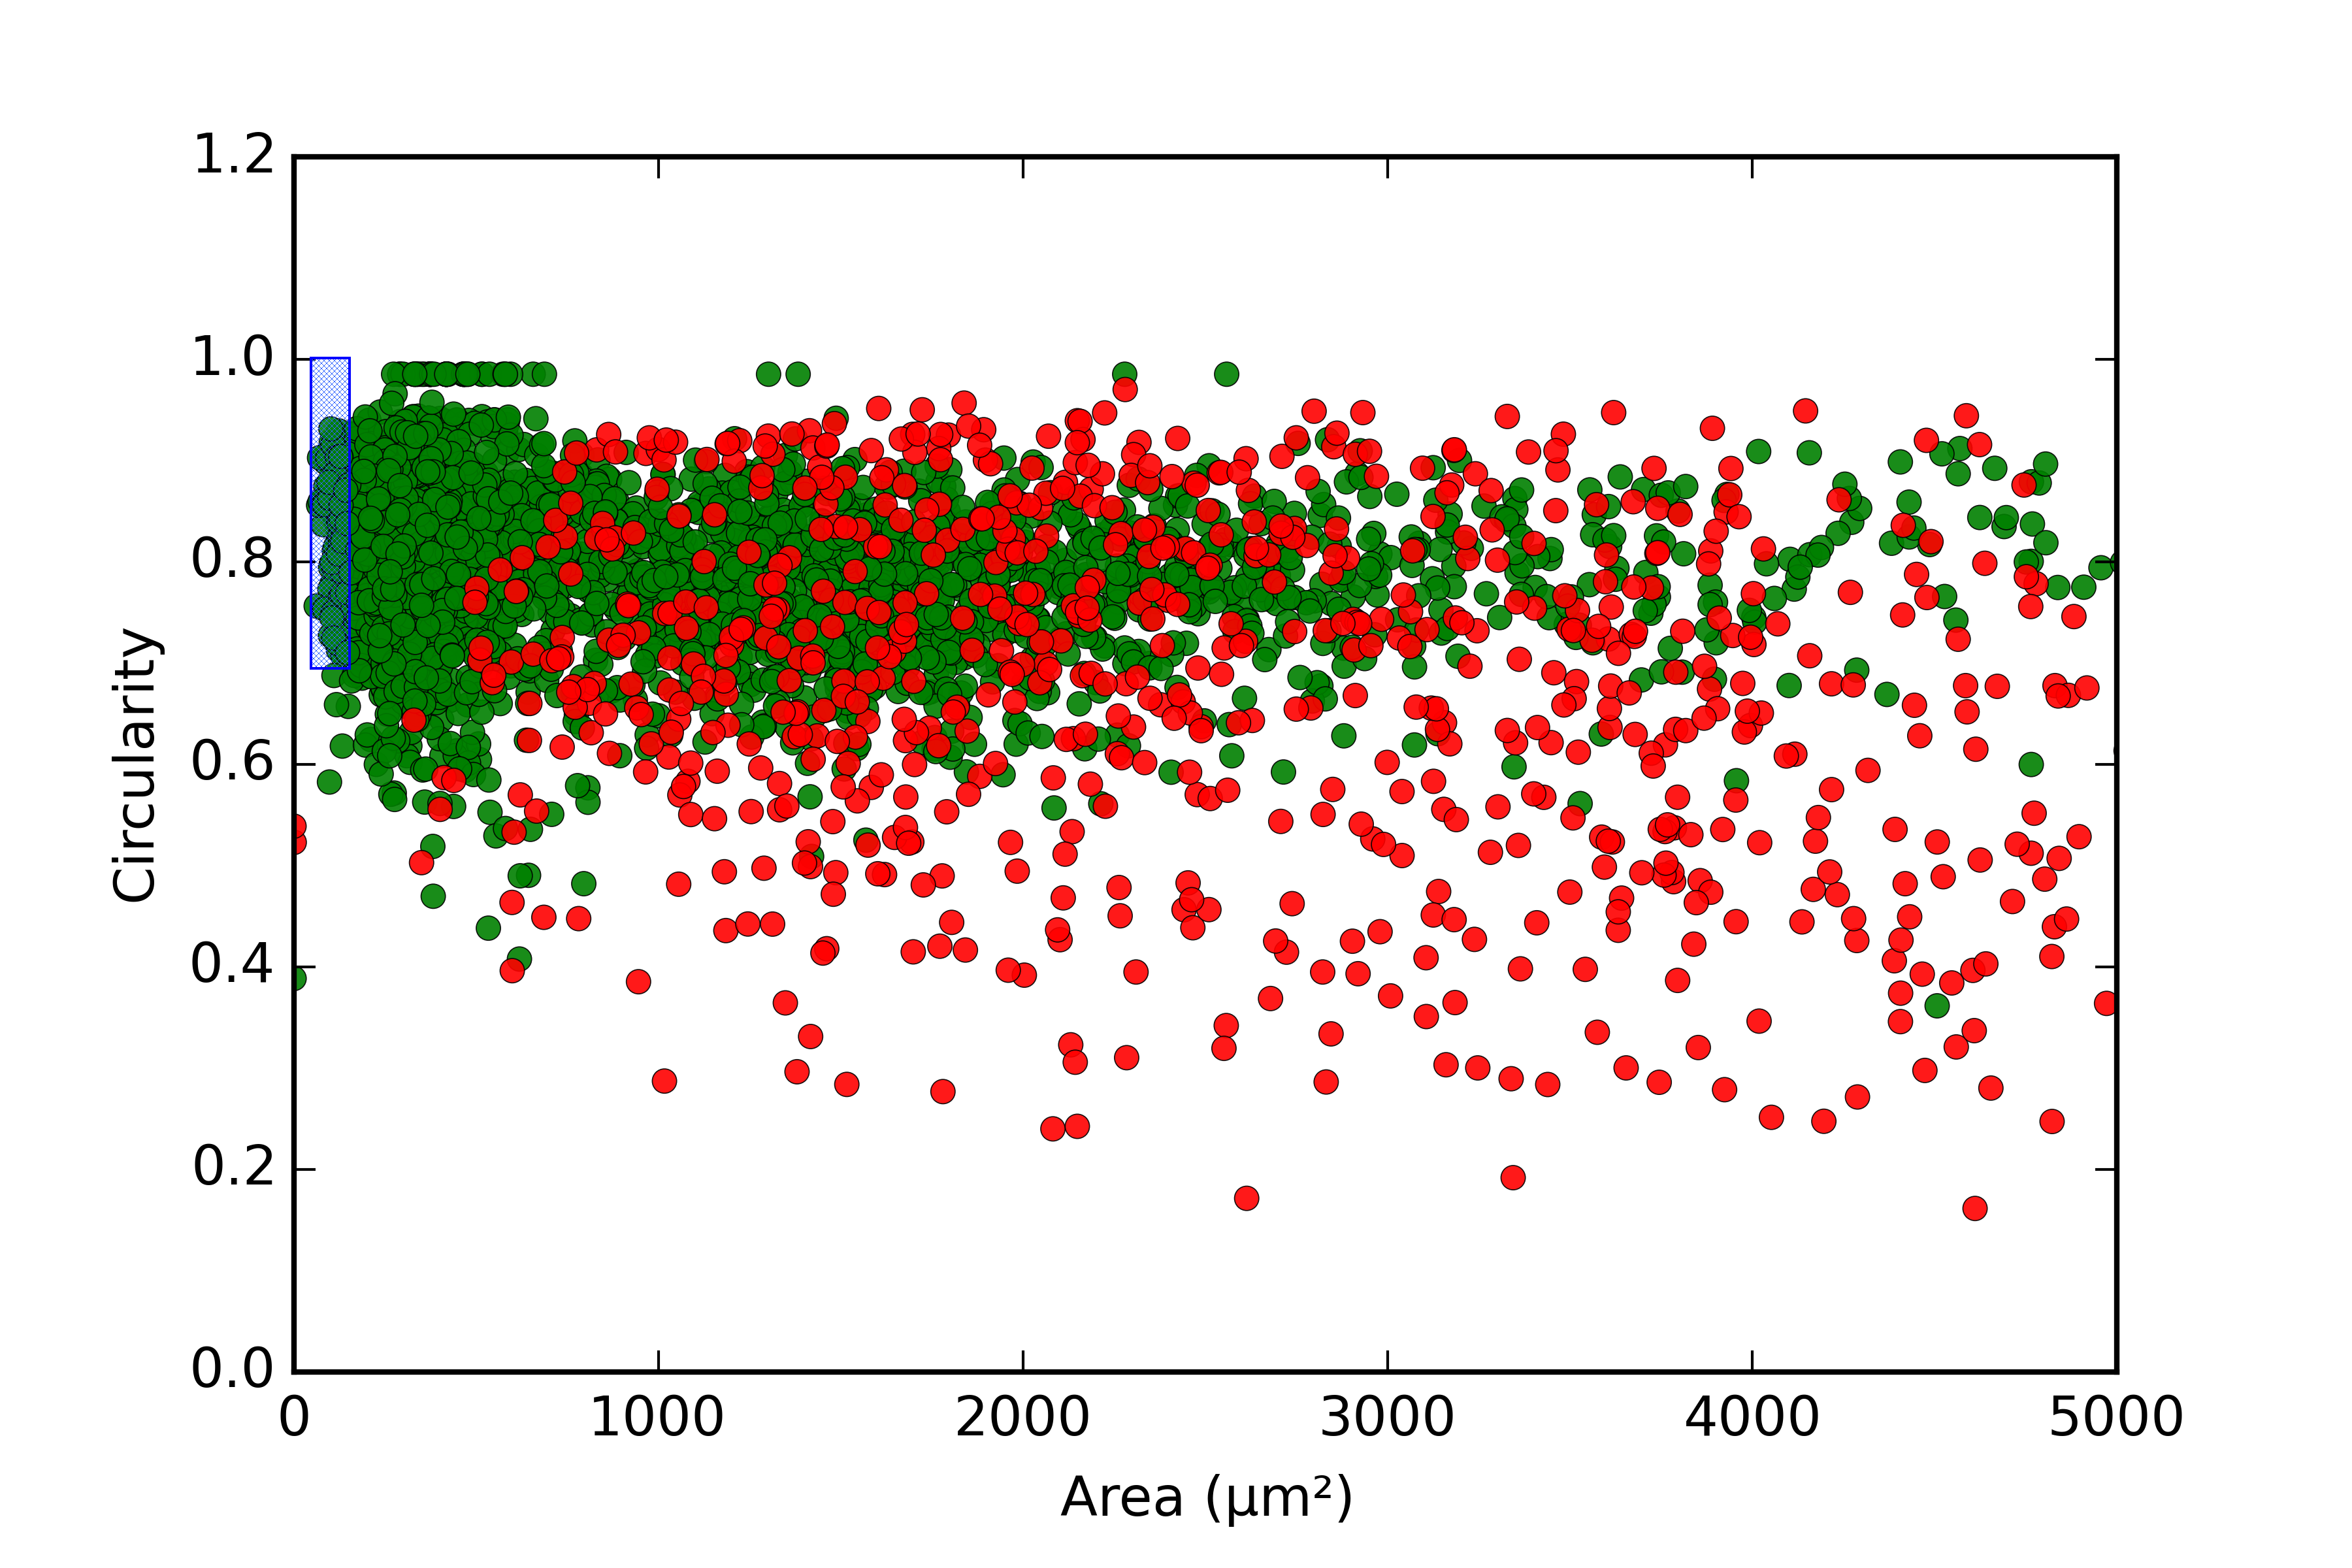
\includegraphics[scale=0.75]{image/scatter_cells_patterns_0_5000.png}
	\caption{Scatter plot, circularity versus area. Green and red dots correspond respectively to cells and patterns. The blue box is the cell dispatching zone.}
	\label{fig:scatter_area_circ_cell_vs_pattern}
\end{figure}

\section{Implementation}
\label{sec:thyroid_implementation}
Actual implementation of the processing using the workflow

\subsection{Seg}
\section{Performance analysis}
\label{sec:thyroid_perf}
\subsection{Detection}
\subsection{Execution times}